Due to the fact that our SFs are defined as a double ratio, we expect some of the systematic uncertainties to cancel at least at first order. Therefore, luminosity, light-lepton and physics modelling uncertainties are expected to be reduced. Unfortunately, tau calibration and MJ background estimation uncertainties do not cancel in the double ratio method. Then, we expect them to dominate the measurement precision.

After calculating the integrated luminosity uncertainty for the SFs, we find that it is less than $0.07\%$, so we just ignore it in our final results. For our uncertainties calculation we use the standard ATLAS procedure. In this method, the objects are re-calibrated using parameters one sigma away from the central value. The results are then compared between the nominal and the re-calibrated events and the difference is quoted as the uncertainty. 

In this chapter the systematic uncertainties for the $Z\to\tauhad\mu$ final state are presented. First for 1-prongs, the uncertainties per source on the C-Factor($Z\to\tauhad \mu$) are shown in Fig. \ref{Fig16a}. For the C-Factor($Z\to\mu\mu$) the same results are shown in Fig. \ref{Fig16b}. After taking the ratio between these two quantities, the uncertainties obtained for the SF are shown in Fig. \ref{Fig16c}. As it can bee seen from the first comparing the first rows of Fig. \ref{Fig16a} and Fig. \ref{Fig16c} the double ratio method helps to reduce the uncertainties coming from the experimental scale factors. Overall, the main uncertainty sources are coming from the jet, MET and tau contributions. The first two directly affect the MET calculation, which in turn has an impact in the estimation of the Z boson mass and the omega variable. The cuts in these variables were re-tuned to mitigate the migration of events out of our selection. For the tau energy scale variations, the problem is that when the $\pT$ of the taus is re-calibrated events can get in our out of the selection. The sensitivity to this effect is correlated with the shape of the $\pT(\tau)$ spectrum. To mitigate this effect a harder cut in $\Delta\phi(\tauhad ,l=\mu , e)$ was put in place. This makes the $\pT(\tau)$ spectrum less rapidly falling. A comparison of the $\pT(\tau)$ shape between two different values for $\Delta\phi(\tauhad ,\mu)$ is shown in Fig. \ref{Fig18}.    

\begin{figure}[htbp]
	\centering
	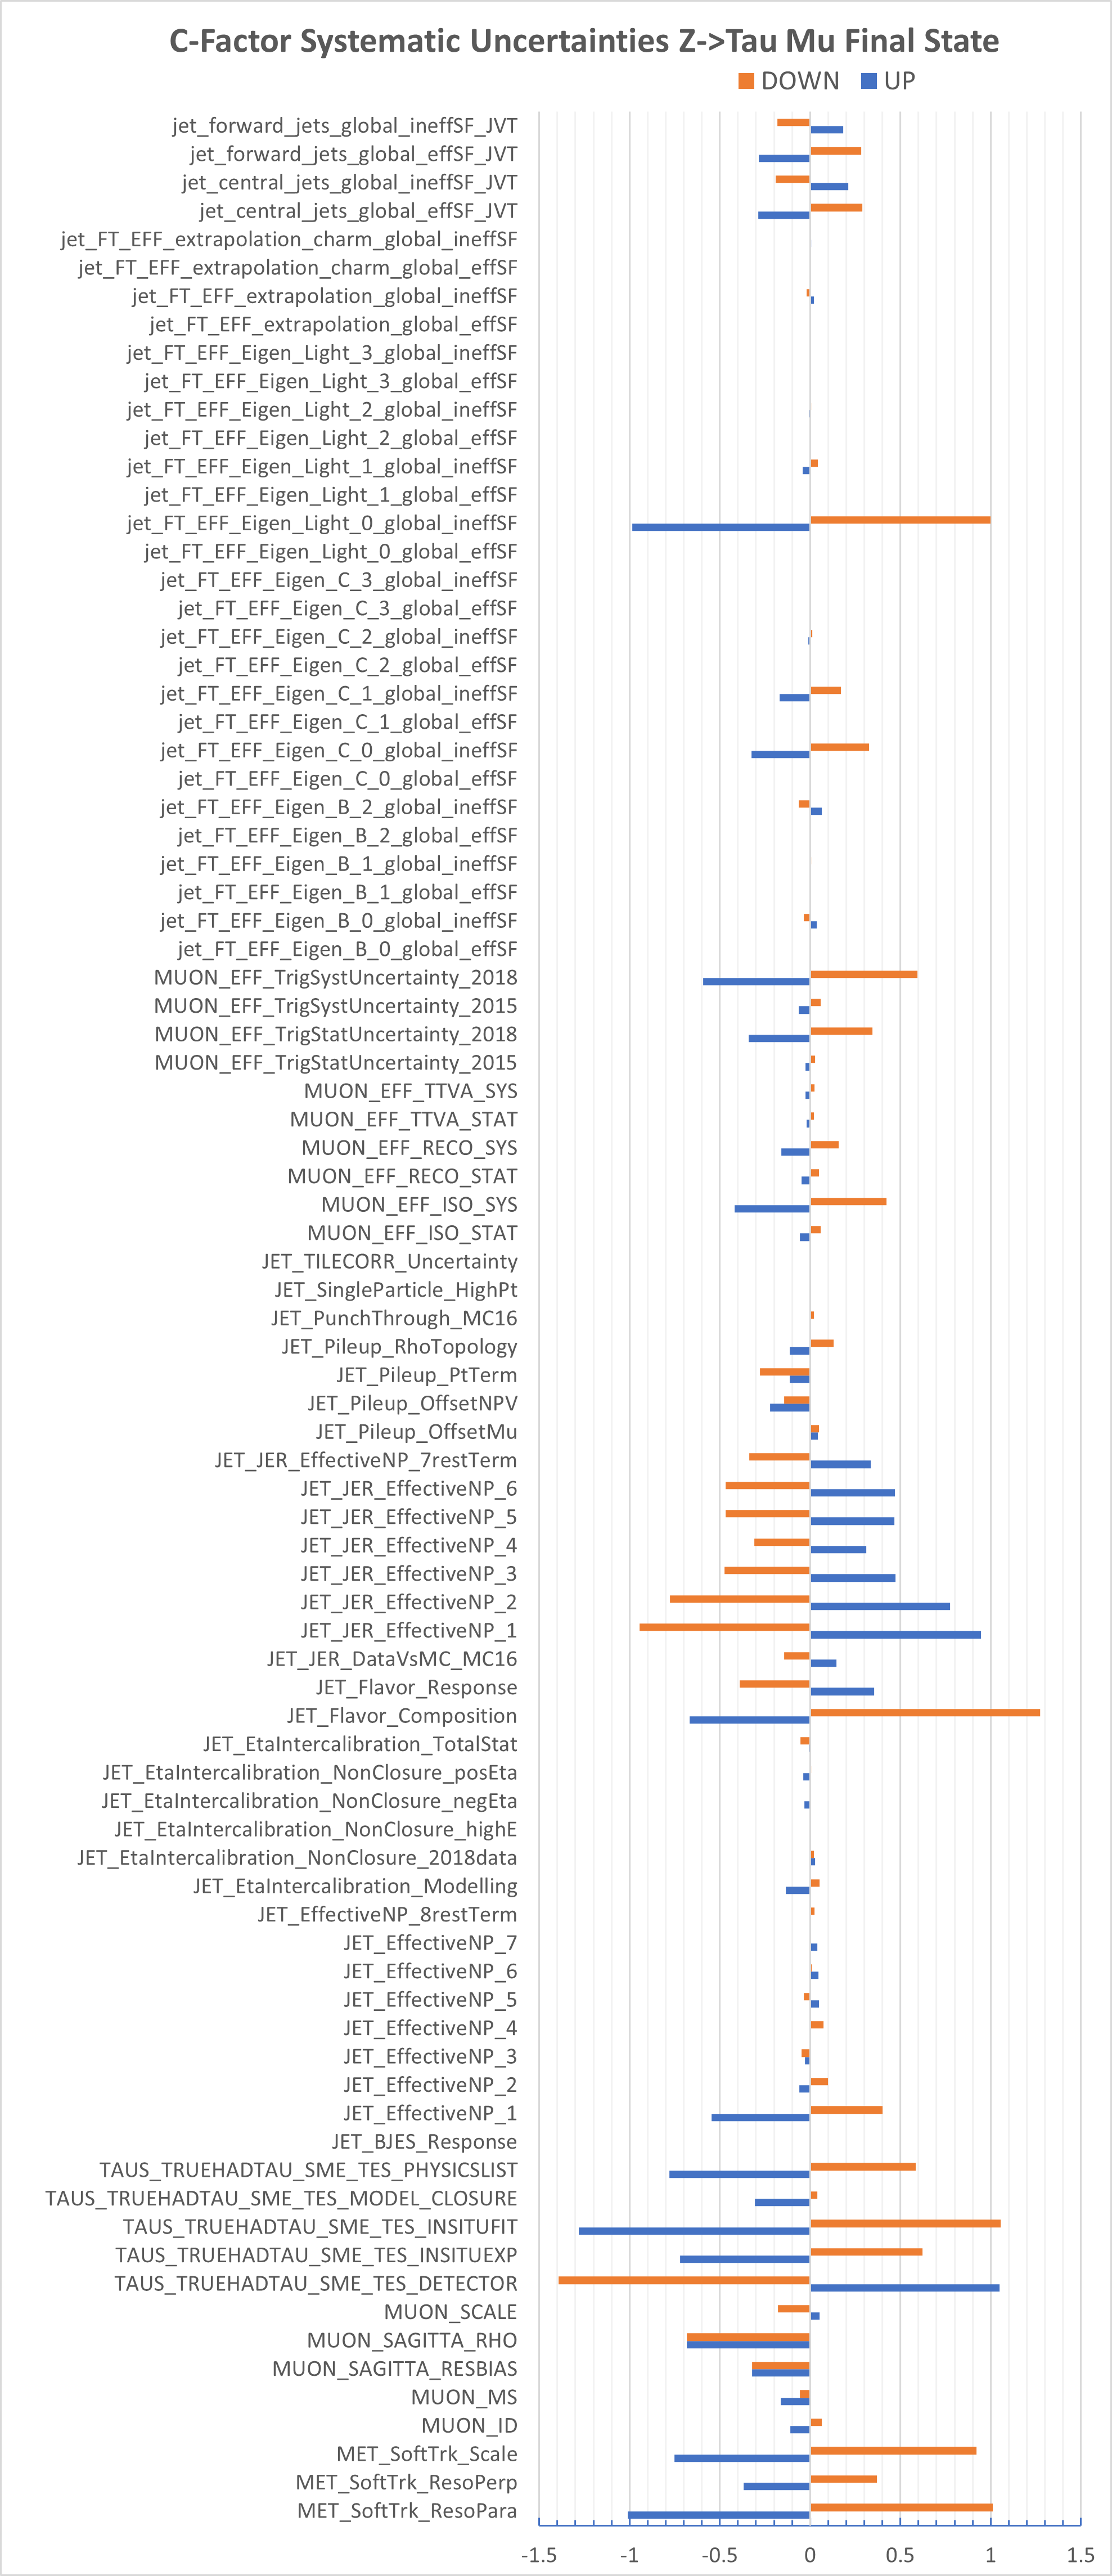
\includegraphics[width=0.5\textwidth]{Fig16a.png}
	\caption{Percentage uncertainties for the C-Factor($Z\to\tauhad\mu$). 1-prong taus.}
	\label{Fig16a}
\end{figure}
\begin{figure}[htbp]
	\centering
	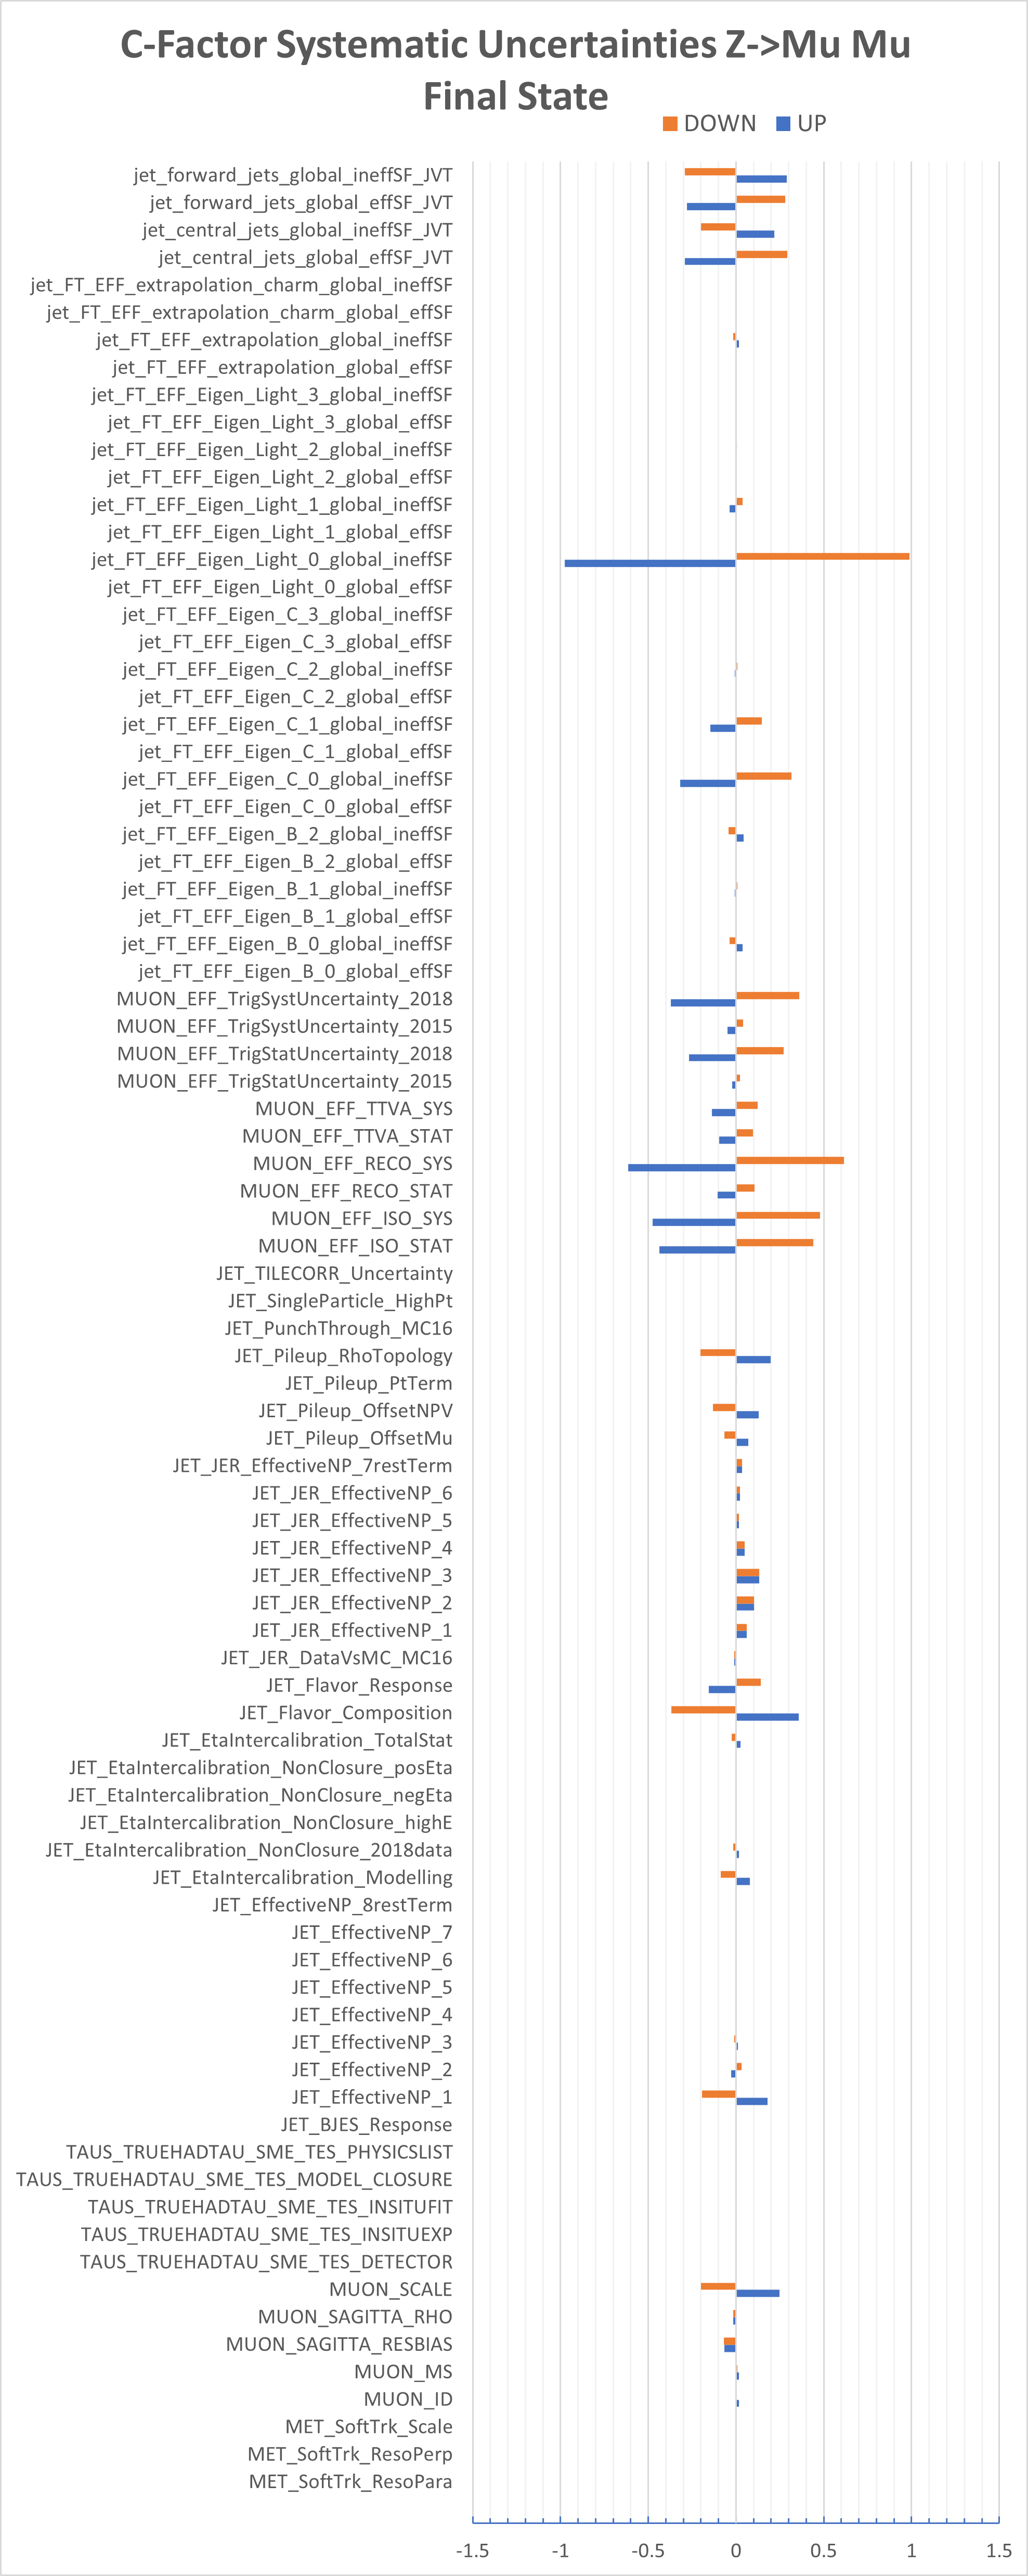
\includegraphics[width=0.5\textwidth]{Fig16b.png}
	\caption{Percentage uncertainties for the C-Factor($Z\to\mu\mu$). 1-prong taus.}
	\label{Fig16b}
\end{figure}
\begin{figure}[htbp]
	\centering
	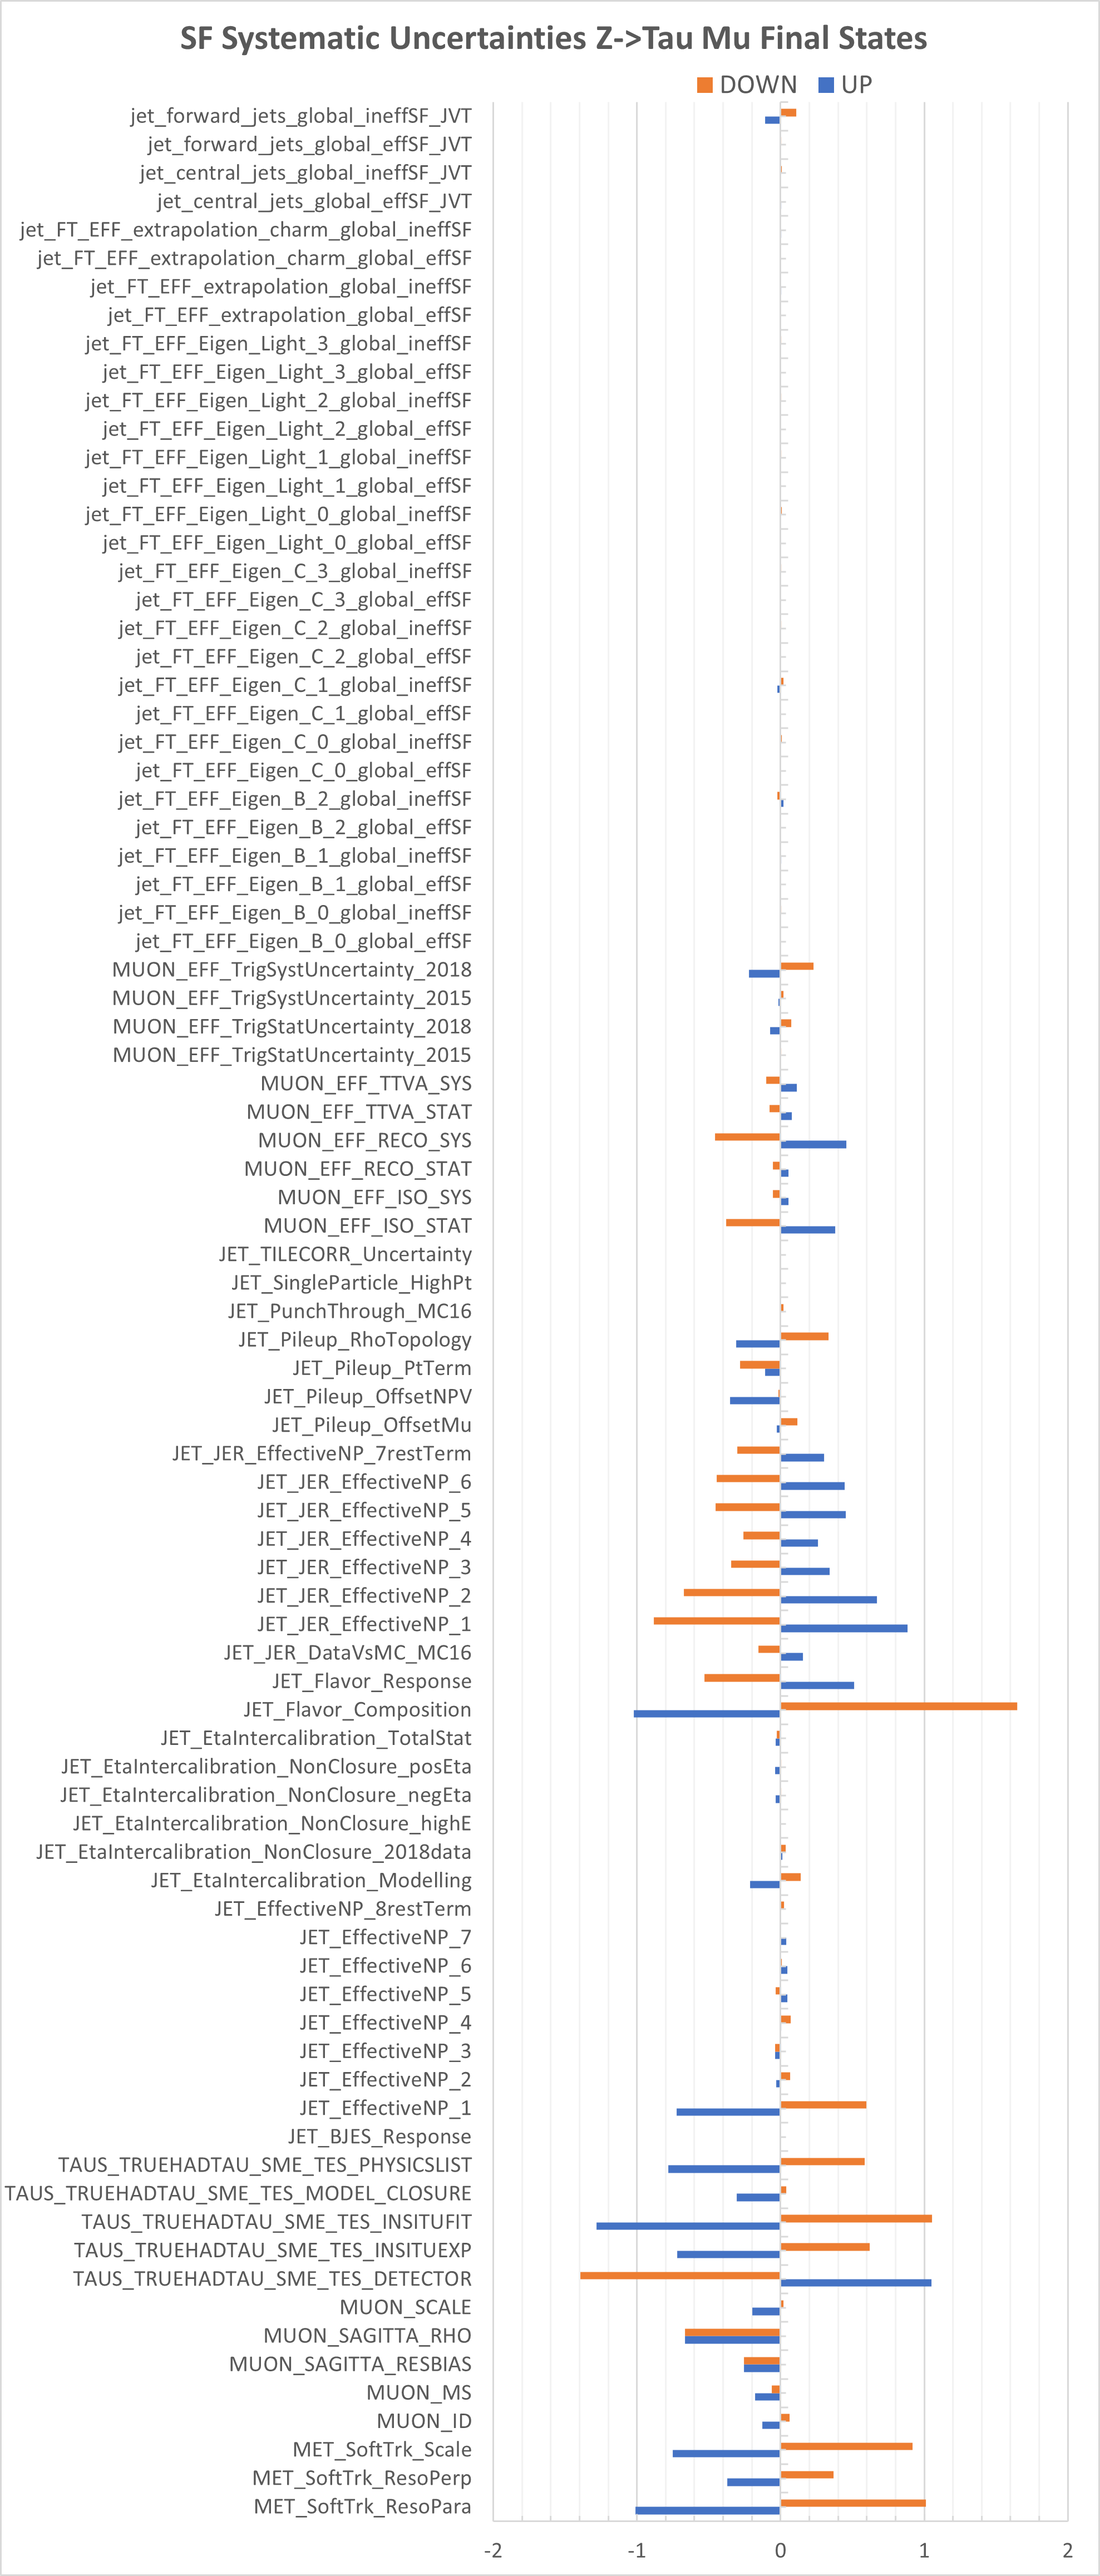
\includegraphics[width=0.5\textwidth]{Fig16c.png}
	\caption{Percentage uncertainties for the SF($Z\to\tauhad\mu$). 1-prong taus.}
	\label{Fig16c}
\end{figure}

\begin{figure}[htbp]
	\centering
	\subfloat[]{\label{Fig18a}{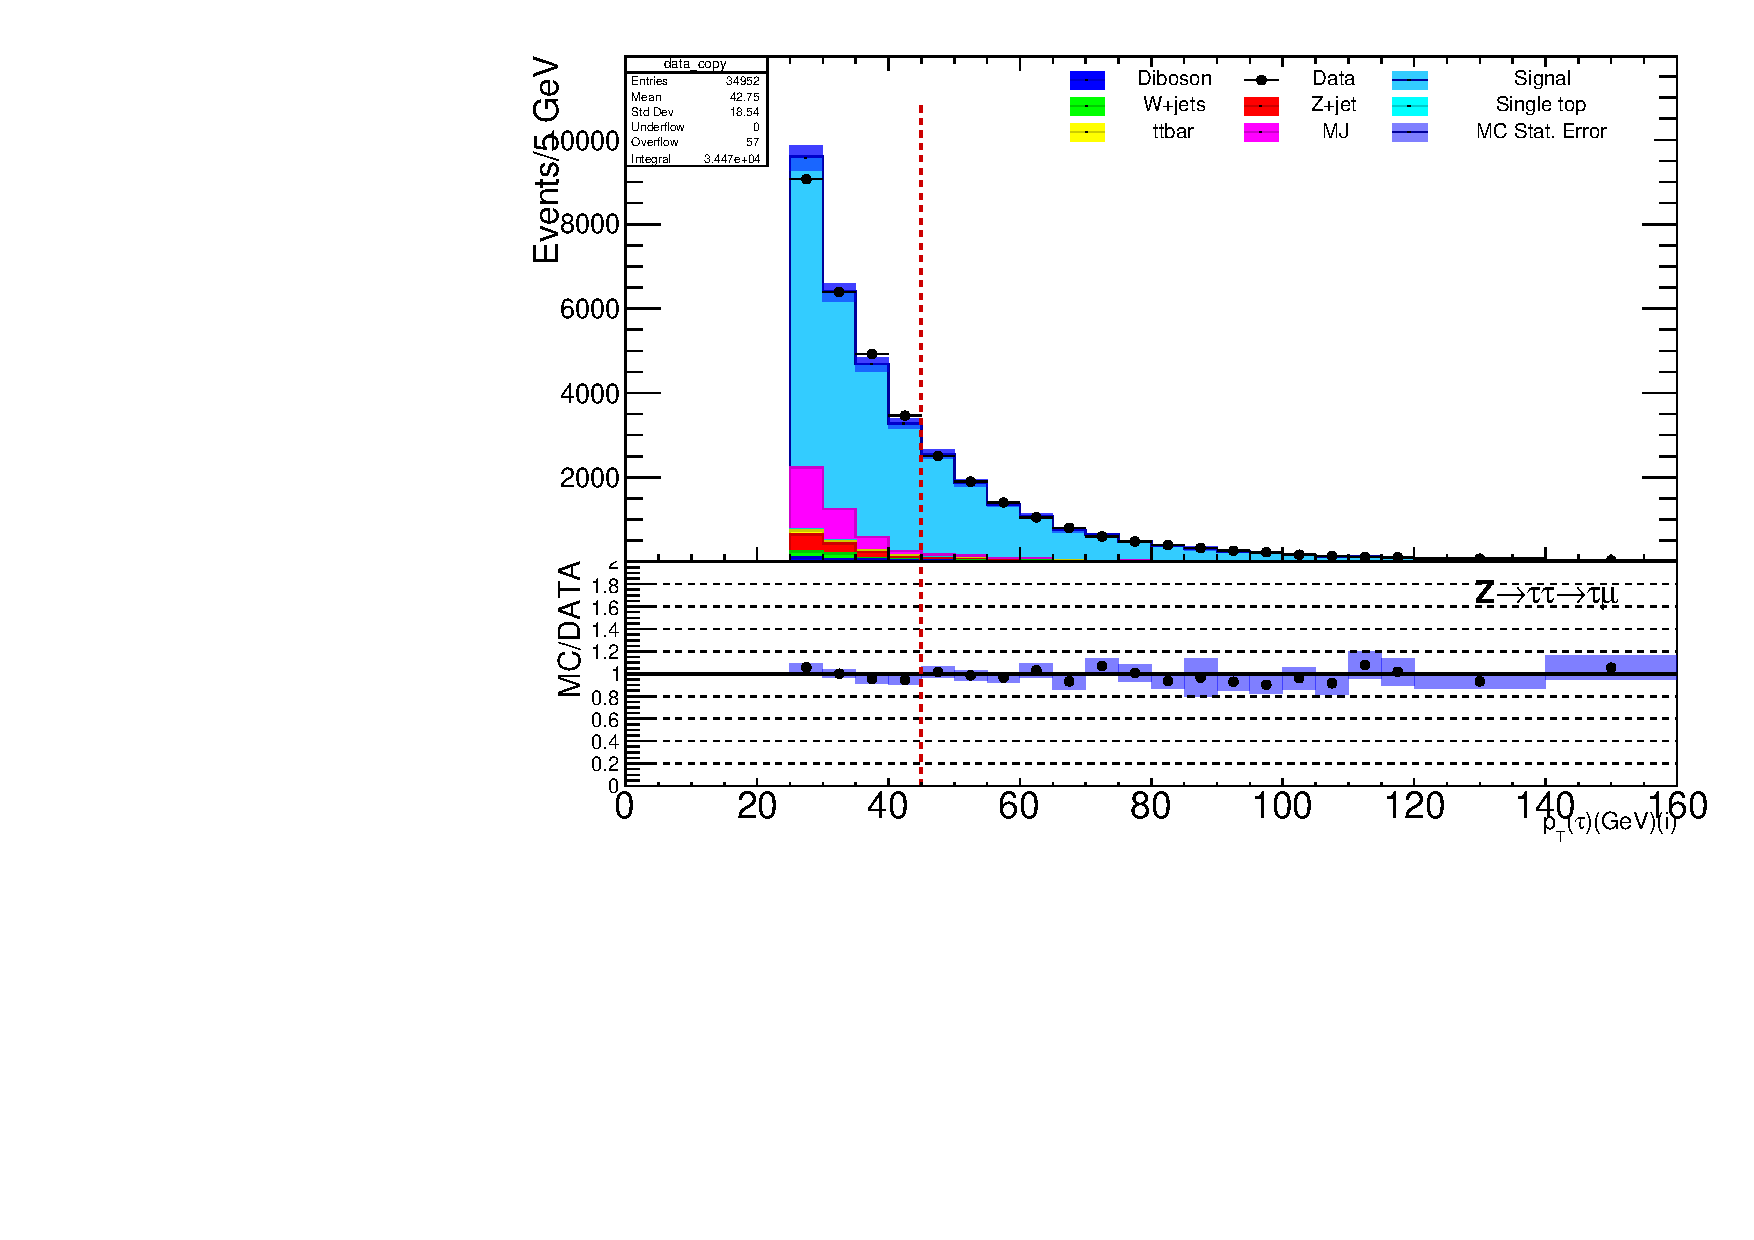
\includegraphics[width=0.50\textwidth]{figures/Fig18a.pdf}}}
	\subfloat[]{\label{Fig18b}{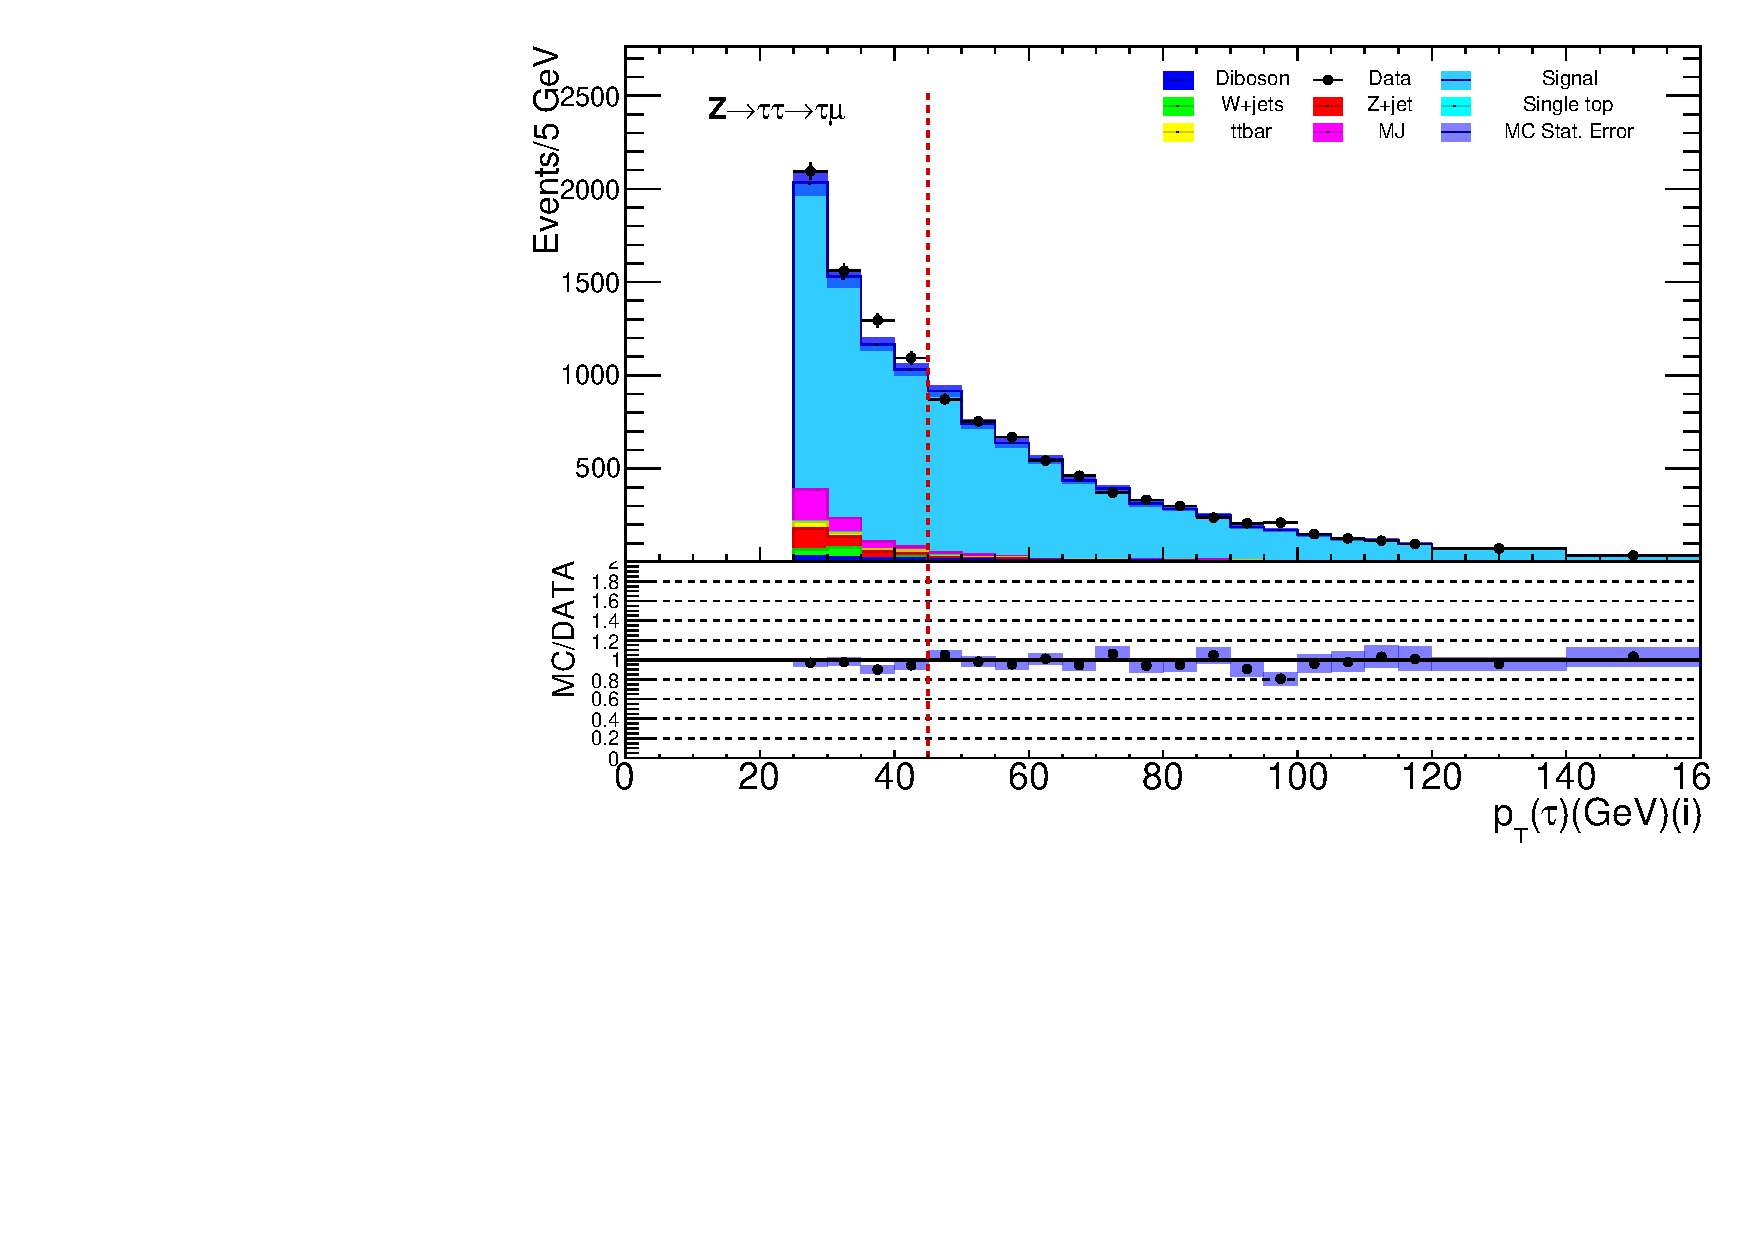
\includegraphics[width=0.50\textwidth]{figures/Fig18b.pdf}}}
	\caption{Figure (a) and (b) show the  $\pT(\tau)$ spectrum for  $\Delta\phi(\tauhad ,\mu)$ less than 1 rad and 2.1 rad respectively. When the harder cut is applied the final $\pT(\tau)$ spectrum falls slower.}
	\label{Fig18}
\end{figure}

For the 3-prongs case the same results are shown in Fig. \ref{Fig17a} and Fig. \ref{Fig17b}.

\begin{figure}[htbp]
	\centering
	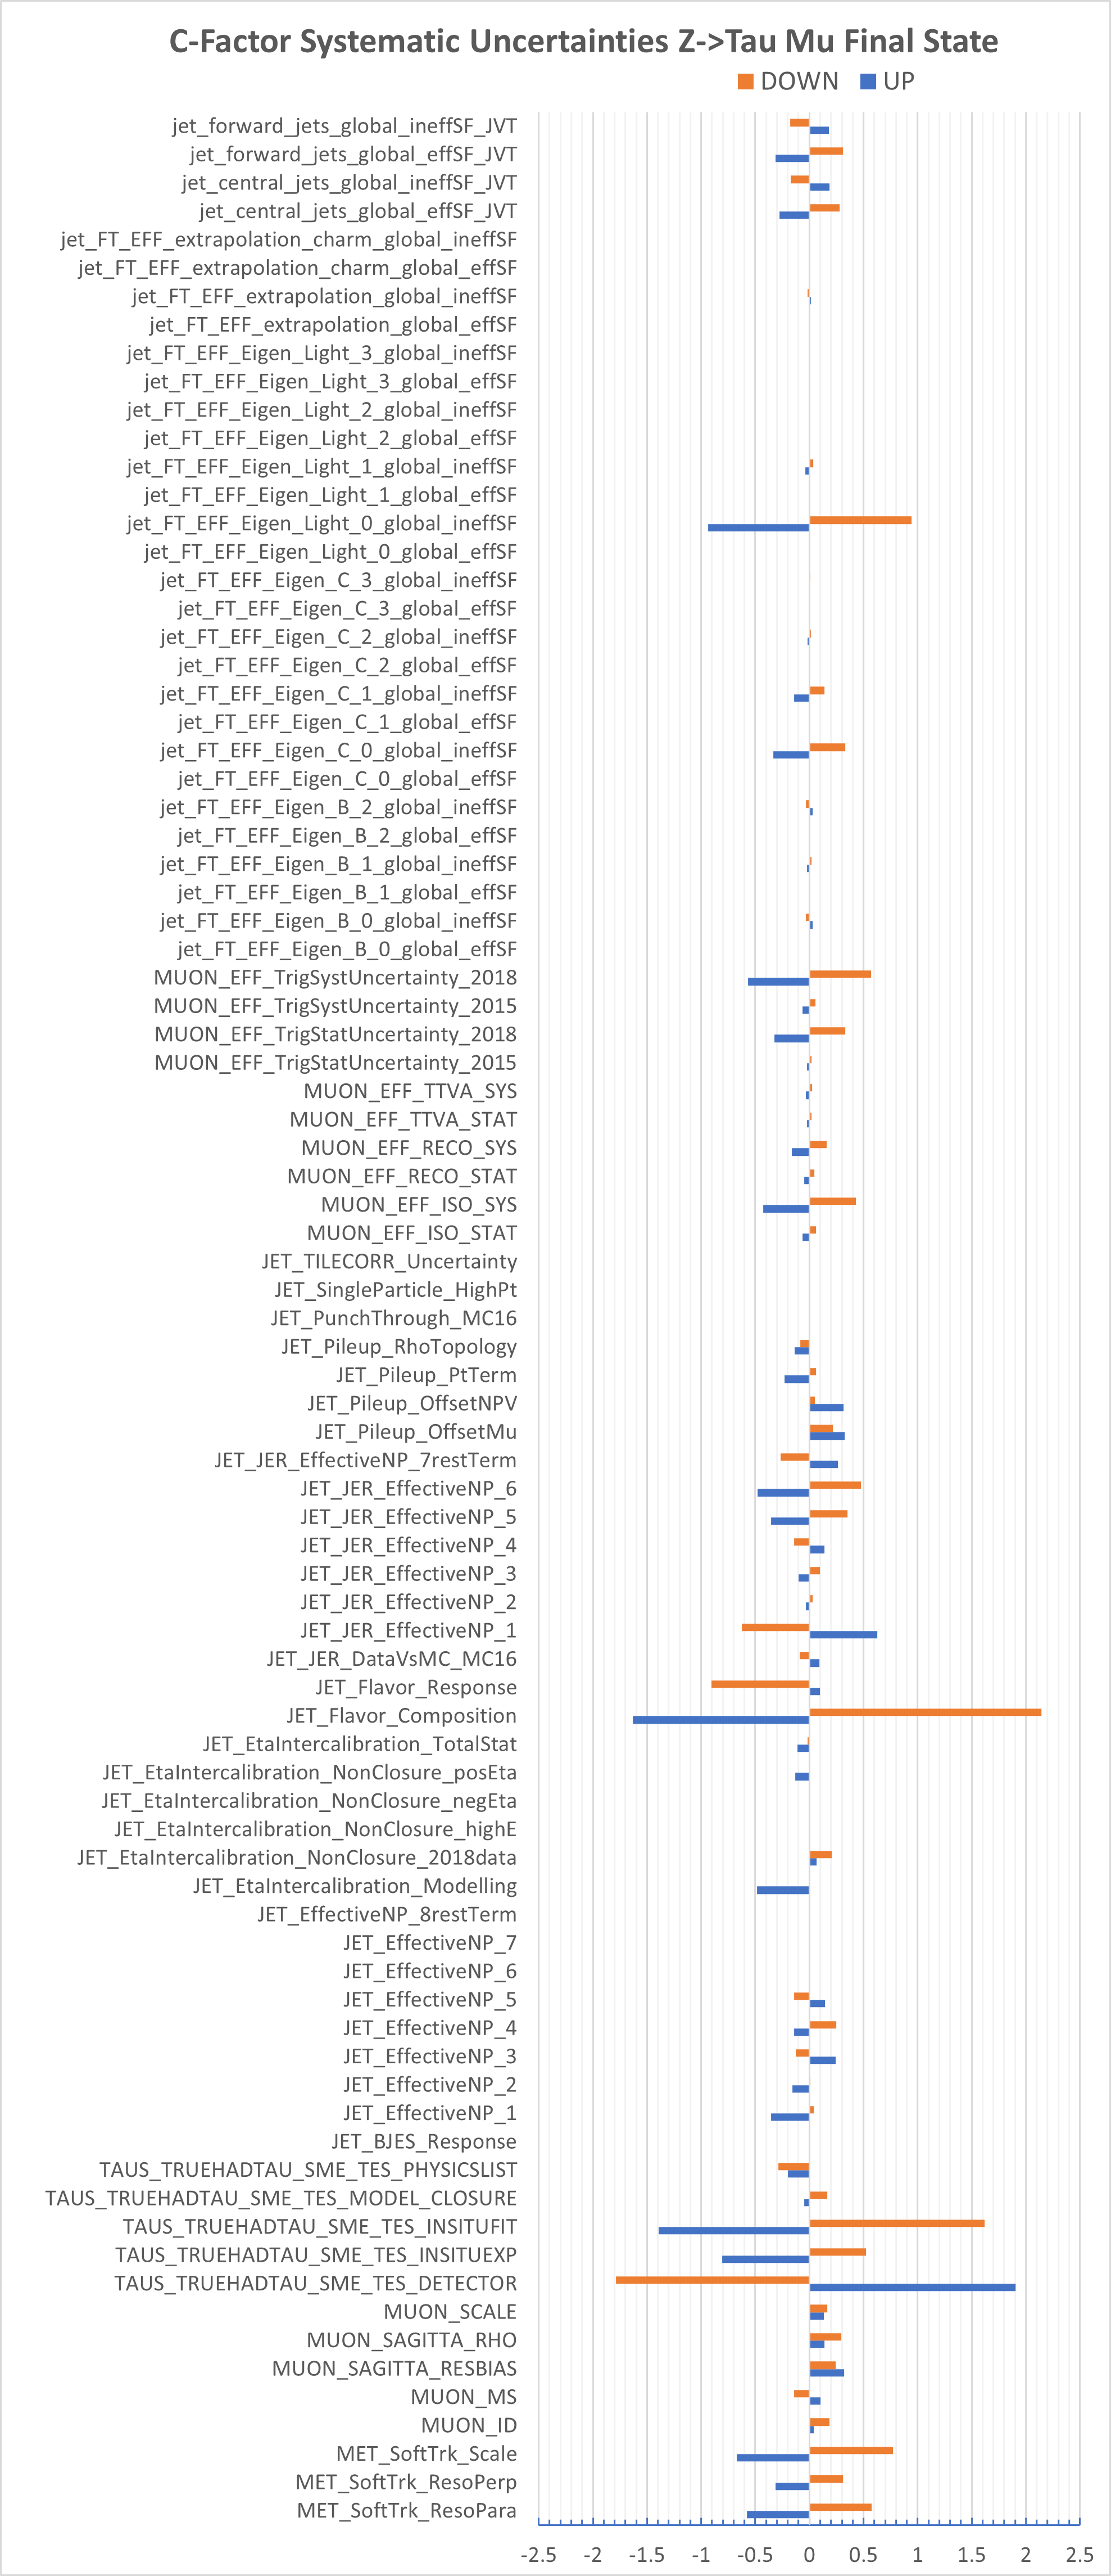
\includegraphics[width=0.5\textwidth]{Fig17a.png}
	\caption{Percentage uncertainties for the C-Factor($Z\to\tauhad\mu$). 3-prong taus.}
	\label{Fig17a}
\end{figure}
\begin{figure}[htbp]
	\centering
	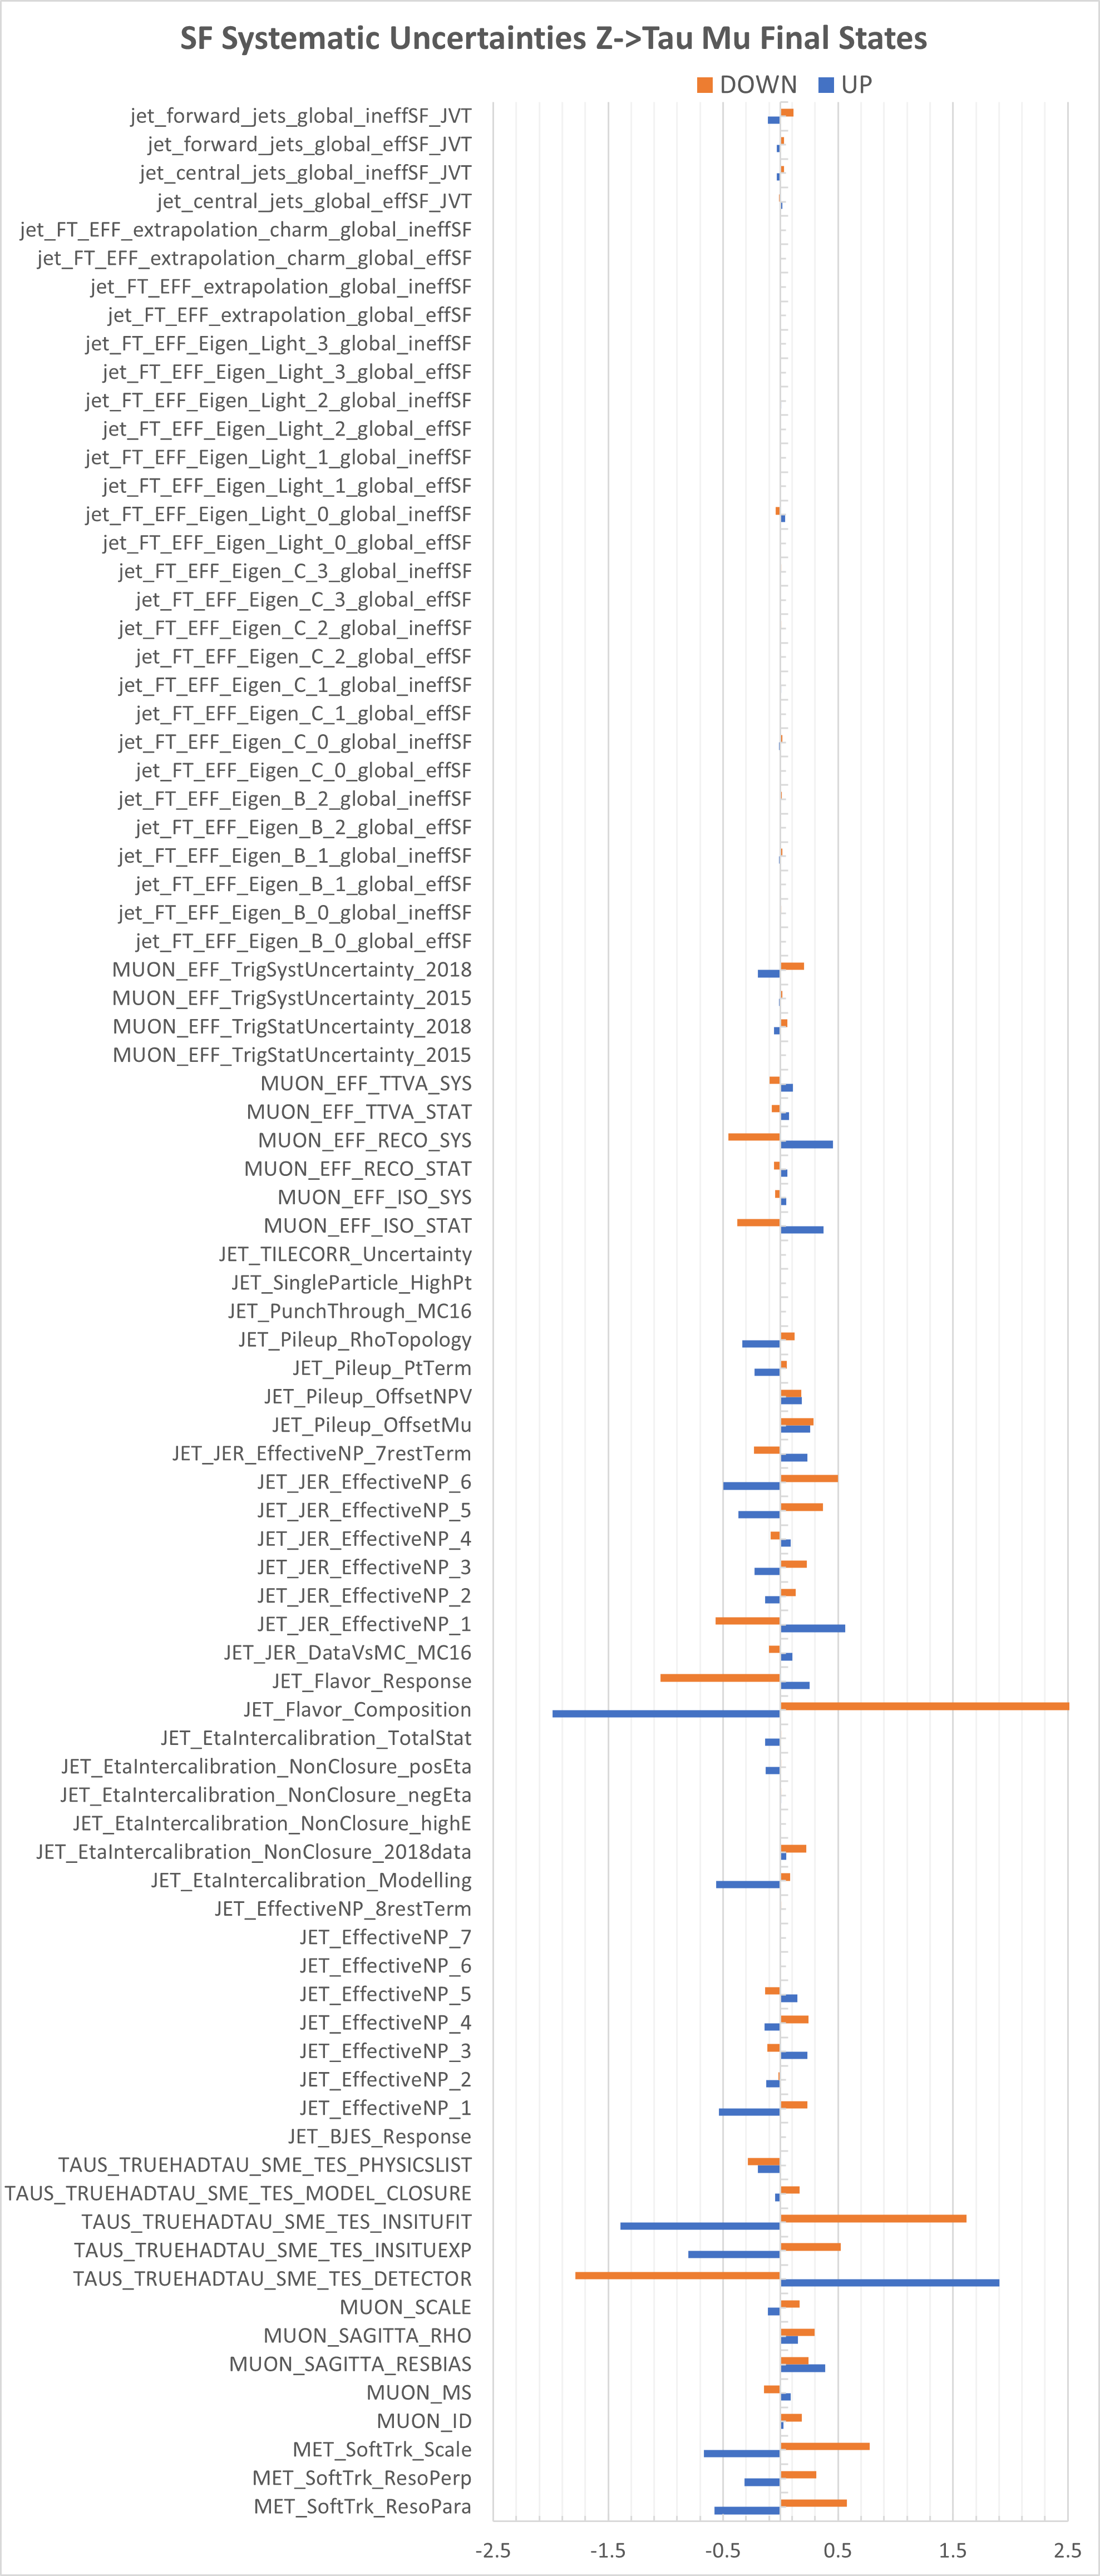
\includegraphics[width=0.5\textwidth]{Fig17b.png}
	\caption{Percentage uncertainties for the SF($Z\to\tauhad\mu$). 3-prong taus.}
	\label{Fig17b}
\end{figure}

Appendix \ref{zteuncer} contains the results for $Z\to\tauhad e$ final state. The conclusions are similar in this case.

Finally, the uncertainties are symmetrized and added in quadrature. The results are summarized in Table. \ref{totalsys} .
\begin{table}[]
	\centering
	\begin{tabular}{|lll|}
		\hline
		\multicolumn{3}{|l|}{1 Prong (\% Syst. Uncertainty)}                         \\ \hline
		\multicolumn{1}{|l|}{Final State}      & \multicolumn{1}{l|}{C-Factor} & SF  \\ \hline
		\multicolumn{1}{|l|}{$Z\to\tauhad\mu$} & \multicolumn{1}{l|}{3.5}      & 3.3 \\ \hline
		\multicolumn{1}{|l|}{$Z\to\tauhad e$}  & \multicolumn{1}{l|}{3.6}      & 3.7 \\ \hline
		\multicolumn{3}{|l|}{3 Prong (\% Syst. Uncertainty)}                         \\ \hline
		\multicolumn{1}{|l|}{$Z\to\tauhad\mu$} & \multicolumn{1}{l|}{3.8}      & 3.8 \\ \hline
		\multicolumn{1}{|l|}{$Z\to\tauhad e$}  & \multicolumn{1}{l|}{4.2}      & 4.2 \\ \hline
	\end{tabular}
	\caption{Total systematic uncertainties given in percentage points.}
	\label{totalsys}
\end{table}